%\documentstyle[epsf,twocolumn]{jarticle}       %LaTeX2e仕様
%\documentclass[twocolumn]{jarticle}     %pLaTeX2e仕様(platex.exeの場合)
\documentclass[onecolumn]{ujarticle}   %pLaTeX2e仕様(uplatex.exeの場合)
%%%%%%%%%%%%%%%%%%%%%%%%%%%%%%%%%%%%%%%%%%%%%%%%%%%%%%%%%%%%%%
%%
%%  基本バージョン
%%
%%%%%%%%%%%%%%%%%%%%%%%%%%%%%%%%%%%%%%%%%%%%%%%%%%%%%%%%%%%%%%%%
\setlength{\topmargin}{-45pt}
%\setlength{\oddsidemargin}{0cm}
\setlength{\oddsidemargin}{-7.5mm}
%\setlength{\evensidemargin}{0cm}
\setlength{\textheight}{24.1cm}
%setlength{\textheight}{25cm}
\setlength{\textwidth}{17.4cm}
%\setlength{\textwidth}{172mm}
\setlength{\columnsep}{11mm}

%\kanjiskip=.07zw plus.5pt minus.5pt


% 【節が変わるごとに (1.1)(1.2) … (2.1)(2.2) と数式番号をつけるとき】
%\makeatletter
%\renewcommand{\theequation}{%
%\thesection.\arabic{equation}} %\@addtoreset{equation}{section}
%\makeatother

%\renewcommand{\arraystretch}{0.95} 行間の設定
%%%%%%%%%%%%%%%%%%%%%%%%%%%%%%%%%%%%%%%%%%%%%%%%%%%%%%%%
%\usepackage{graphicx}   %pLaTeX2e仕様(\documentstyle ->\documentclass)
\usepackage[dvipdfmx]{graphicx}
\usepackage{subcaption}
\usepackage{multirow}
\usepackage{amsmath}
\usepackage{url}
\usepackage[bb=boondox]{mathalfa}
\newcommand{\argmax}{\mathop{\rm arg~max}\limits}
\newcommand{\argmin}{\mathop{\rm arg~min}\limits}
%%%%%%%%%%%%%%%%%%%%%%%%%%%%%%%%%%%%%%%%%%%%%%%%%%%%%%%%
\begin{document}

	%bibtex用の設定
	%\bibliographystyle{ujarticle}
	\noindent

	\hspace{1em}
	2020 年 6 月 19 日
	ゼミ資料
	\hfill
	M2 寺内 光

	\vspace{2mm}

	\hrule

	\begin{center}
		{\Large \bf 進捗報告}
	\end{center}

	\hrule
	\vspace{3mm}

	% ‚ここから 文章 Start!
	\section{今週やったこと}
	\begin{itemize}{
		\item{TDGA実装,ドキュメンテーション,論文追実験}
	}\end{itemize}

	\section{TDGA実装,ドキュメンテーション}
	TDGA の遺伝子型として整数をとれるように拡張して実装.\url{https://github.com/1g-hub/TDGA} においてます.
	コードレビュー会しましょう(忘れる前に).

	\section{論文の追実験}
	まずは各アルゴリズムについて突然変異率および個体数を変化させて,それぞれの場合について乱数の初期値を変えて 30 荷物のナップサック問題を 各 30 回ずつ解かせ,100 世代以内に最適解を得た回数を調べる.
	表 \ref{tab:items} に用いた荷物及び制約を示す.
	\begin{figure}[h]
		\begin{center}
			\caption{The 30-item knapsack problem}
			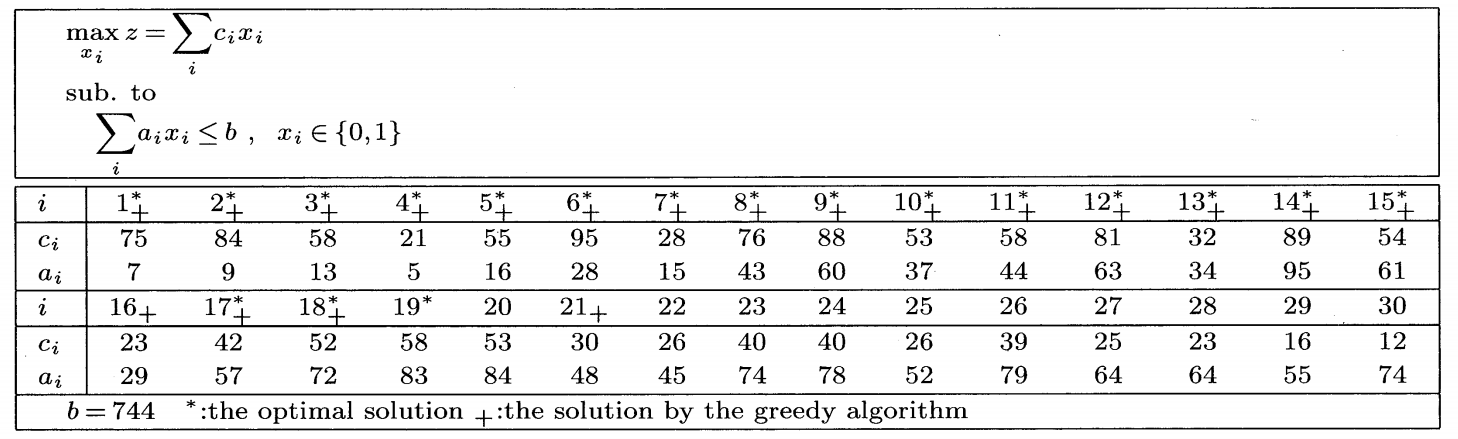
\includegraphics[width=1.0\columnwidth]{figure/knapsackitems.png}
			\label{tab:items}
		\end{center}
	\end{figure}

	図 \ref{fig:variousmute} に個体数を TDGA では 32, SGA では 64 とし,突然変異率を変化させた場合の結果を示す.

	\begin{figure}[h]
		\vspace{-20mm}
		\begin{center}
			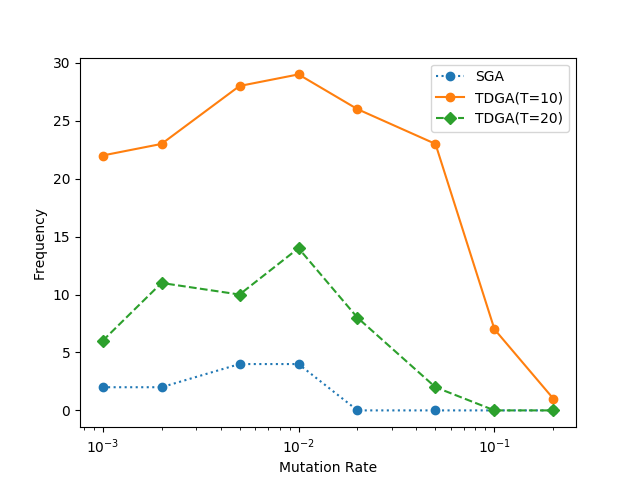
\includegraphics[width=0.7\columnwidth]{figure/exp_mut.png}
			\caption{Comparison of TDGA and SGA with various mutation rates}
			\label{fig:variousmute}
		\end{center}
	\end{figure}

	SGA が論文より精度が出ないのでどこかしらかに実装の違いがありそう.

	図 \ref{fig:variousNp} に個体数を変化させた場合の結果を示す.突然変異率は図 \ref{fig:variousmute} で最も良い結果を出している値(0.01)を使用する.

	\begin{figure}[h]
		\begin{center}
			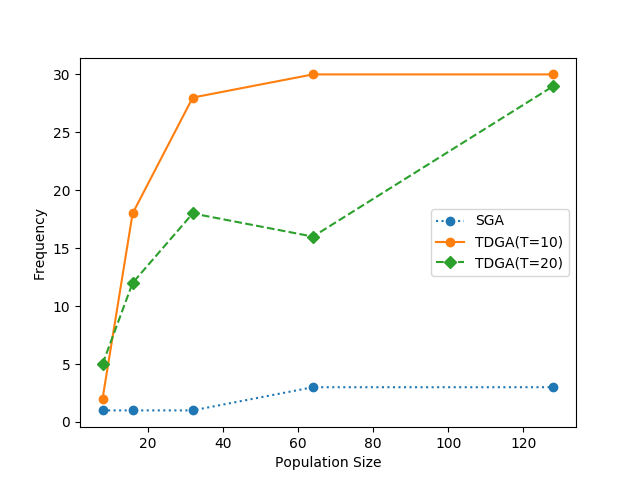
\includegraphics[width=0.7\columnwidth]{figure/exp_Np.png}
			\caption{Comparison of TDGA and SGA with various population sizes}
			\label{fig:variousNp}
		\end{center}
	\end{figure}

	また,突然変異率が 0.01, 個体数 32(SGA では 64)の場合の探索の様子を 図 \ref{fig:searchprocessT10}, \ref{fig:searchprocessT20}, \ref{fig:searchprocessSGA} に示す.各図の横軸は世代,縦軸は目的関数値を表す.このときの多様性の維持の様子を,各世代での遺伝子座毎のエントロピーを用いて図 \ref{fig:entropyT10}, \ref{fig:entropyT20}, \ref{fig:entropySGA} に示す.三つの軸はそれぞれ遺伝子座,世代およびエントロピーを表す.また,SGA の突然変異率を変化させたものを載せる.

	\begin{figure}[h]
		\vspace{-8mm}
		\begin{subfigure}{0.49\columnwidth}
			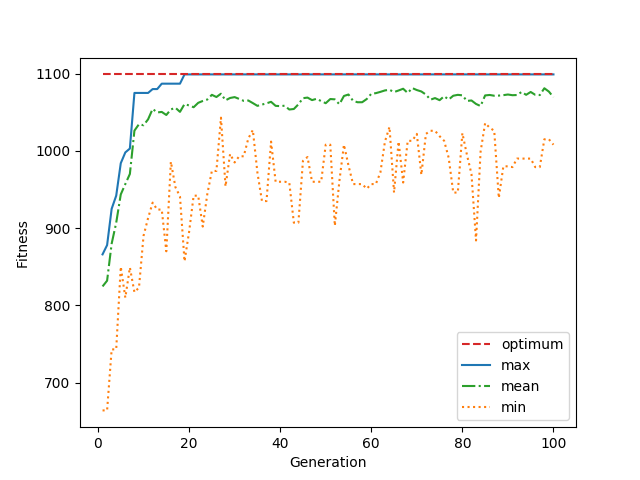
\includegraphics[width=1.0\columnwidth]{figure/knapsackTDGA_stats_T_10_mut_001_Np_32.png}
			\caption{Search process of the TDGA($T$=10)}
			\label{fig:searchprocessT10}
		\end{subfigure}
		\begin{subfigure}{0.49\columnwidth}
			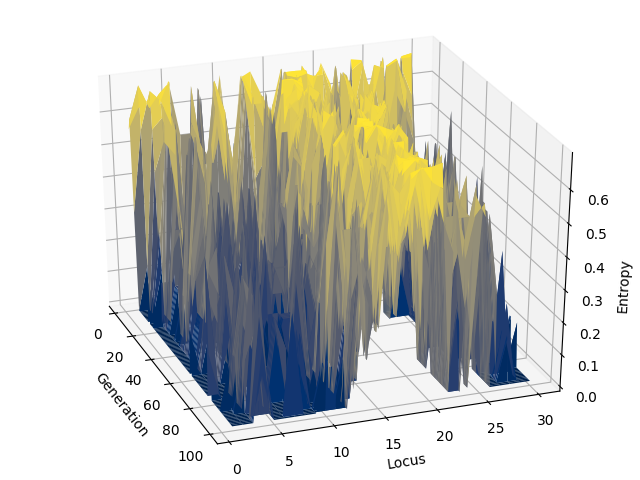
\includegraphics[width=1.0\columnwidth]{figure/knapsackTDGA_T_10_mut_001_Np_32.png}
			\caption{Variation of the entropy of each locus in case of the TDGA($T$=10)}
			\label{fig:entropyT10}
		\end{subfigure}
		\caption{Experiment of the TDGA($T$=10)}
	\end{figure}

	\begin{figure}[h]
		\vspace{-2mm}
		\begin{subfigure}{0.49\columnwidth}
			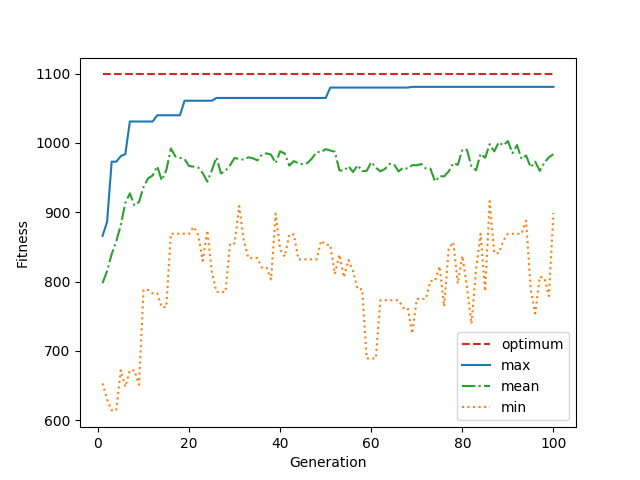
\includegraphics[width=1.0\columnwidth]{figure/knapsackTDGA_stats_T_20_mut_001_Np_32.png}
			\caption{Search process of the TDGA($T$=20)}
			\label{fig:searchprocessT20}
		\end{subfigure}
		\begin{subfigure}{0.49\columnwidth}
			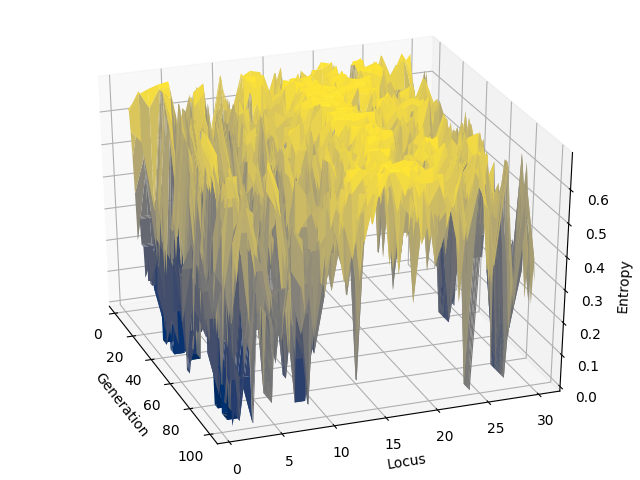
\includegraphics[width=1.0\columnwidth]{figure/knapsackTDGA_T_20_mut_001_Np_32.png}
			\caption{Variation of the entropy of each locus in case of the TDGA($T$=20)}
			\label{fig:entropyT20}
		\end{subfigure}
		\caption{Experiment of the TDGA($T$=20)}
	\end{figure}

	\begin{figure}[h]
		\begin{subfigure}{0.49\columnwidth}
			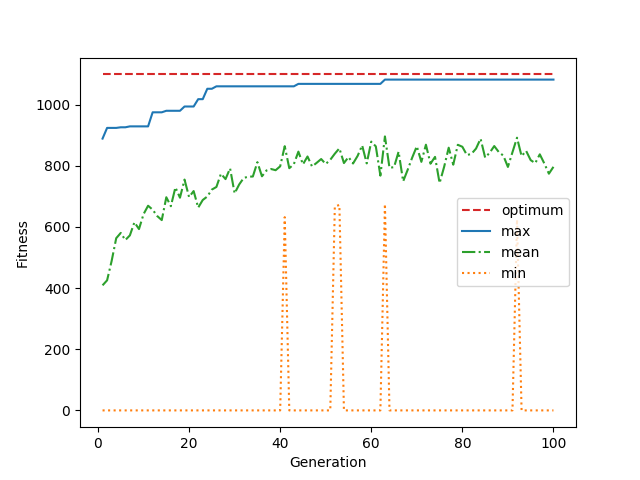
\includegraphics[width=1.0\columnwidth]{figure/knapsackSGA_stats_mut_001_Np_64.png}
			\caption{Search process of the SGA(mutation pr=0.01)}
			\label{fig:searchprocessSGA}
		\end{subfigure}
		\begin{subfigure}{0.49\columnwidth}
			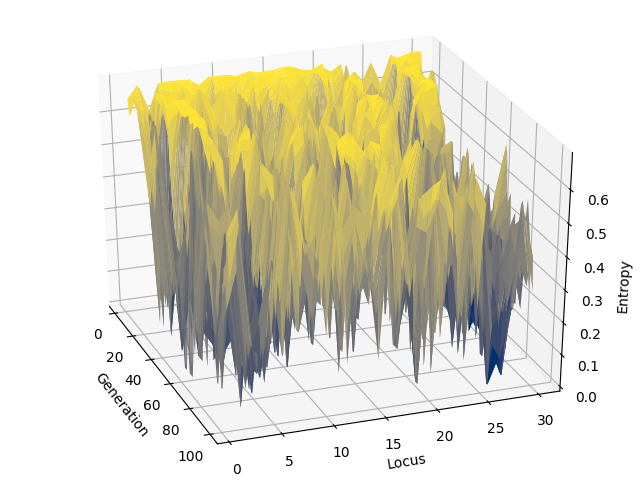
\includegraphics[width=1.0\columnwidth]{figure/knapsackSGA_mut_001_Np_64.png}
			\caption{Variation of the entropy of each locus in case of the SGA(mutation pr=0.01)}
			\label{fig:entropySGA}
		\end{subfigure}
		\caption{Experiment of the SGA(mutation pr=0.01)}
	\end{figure}

	\begin{figure}[h]
		\begin{subfigure}{0.49\columnwidth}
			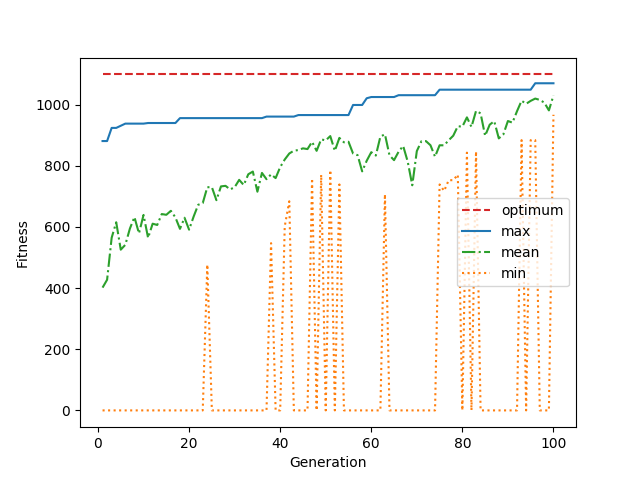
\includegraphics[width=1.0\columnwidth]{figure/knapsackSGA_stats_mut_0002_Np_64.png}
			\caption{Search process of the SGA(mutation pr=0.002)}
			\label{fig:searchprocessSGApr0002}
		\end{subfigure}
		\begin{subfigure}{0.49\columnwidth}
			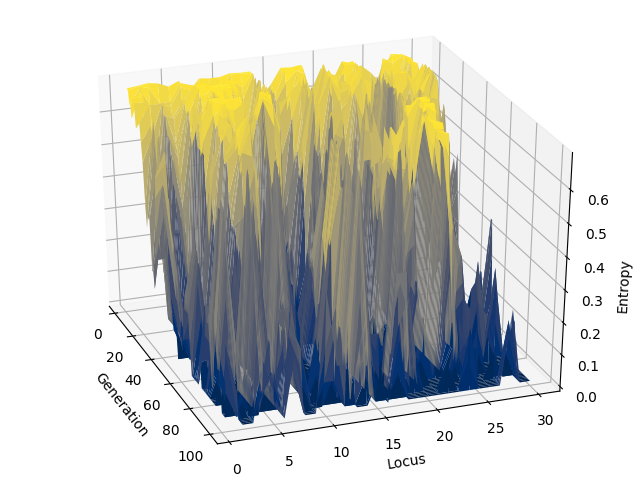
\includegraphics[width=1.0\columnwidth]{figure/knapsackSGA_mut_0002_Np_64.png}
			\caption{Variation of the entropy of each locus in case of the SGA(mutation pr=0.002)}
			\label{fig:entropySGApr0002}
		\end{subfigure}
		\caption{Experiment of the SGA(mutation pr=0.002)}
	\end{figure}

	\begin{figure}[h]
		\begin{subfigure}{0.49\columnwidth}
			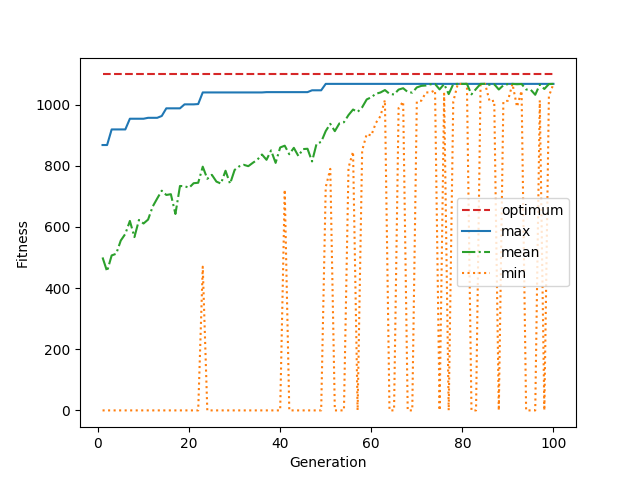
\includegraphics[width=1.0\columnwidth]{figure/knapsackSGA_stats_mut_0001_Np_64.png}
			\caption{Search process of the SGA(mutation pr=0.001)}
			\label{fig:searchprocessSGApr0001}
		\end{subfigure}
		\begin{subfigure}{0.49\columnwidth}
			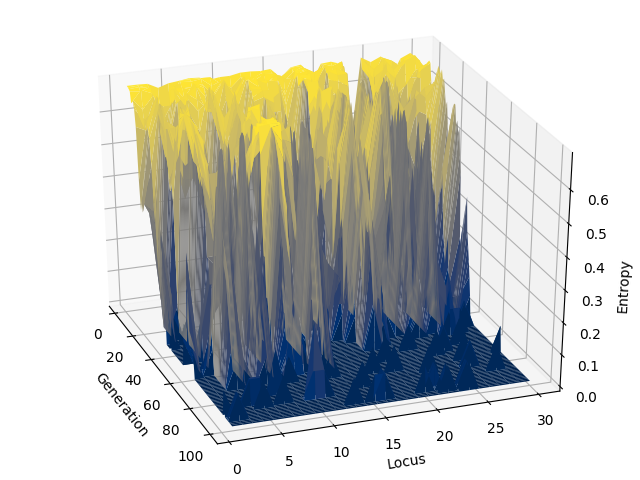
\includegraphics[width=1.0\columnwidth]{figure/knapsackSGA_mut_0001_Np_64.png}
			\caption{Variation of the entropy of each locus in case of the SGA(mutation pr=0.001)}
			\label{fig:entropySGApr0001}
		\end{subfigure}
		\caption{Experiment of the SGA(mutation pr=0.001)}
	\end{figure}

	TDGA は概ね良さそう.SGA においては論文中でも突然変異率を下げて収束していたので収束という点では問題なさそう(収束突然変異率が少し小さいのが気にはなるが).現状, SGA の min が 0 のままなのが論文との1番の相違点.
	表 \ref{tab:exp_condition_SGA} に SGA の実験設定を示す.

	\begin{table}[h]
		\centering
		\caption{SGA 実験条件}
		\label{tab:exp_condition_SGA}
		\begin{tabular}{|c||c|} \hline
			交叉&一様交叉($p$=0.5)\\ \hline
			突然変異&ビット反転($p$=0.002)\\ \hline
			選択&適応度比例戦略(ルーレット選択)+エリート保存\\ \hline
			スケーリング&線形スケーリング($A=3$, $B=1$)\\ \hline
			個体数&64\\ \hline
			世代数&100\\ \hline
		\end{tabular}
	\end{table}


	\section{来週のタスク}
	前期発表会の準備.

	% 参考文献リスト
	% \bibliographystyle{unsrt}
	% \bibliography{2020_06_19}
\end{document}
